%%---------------------------------------------------------------------
%	Preamble
%	AMS gruppe 12
%	AMS F18
%---------------------------------------------------------------------
\documentclass[12pt,fleqn,a4paper]{article}
\usepackage[utf8]{inputenc}
\usepackage[danish]{babel}
\usepackage[top=2.5cm, left=2cm, right=2cm, bottom=2.5cm]{geometry}
\usepackage{graphicx}
\usepackage[bottom]{footmisc}
\usepackage{framed}
\usepackage{caption}
\usepackage{float}
\usepackage{mdframed}
\usepackage{listings}
\usepackage{color}
\usepackage[T1]{fontenc}
\usepackage{amsmath,amsfonts,amsthm} % Math packages
\usepackage{array}
\usepackage{wrapfig}
\usepackage{multirow}
\usepackage{tabu}
\usepackage{longtable}
\usepackage{lastpage}
\usepackage{fancyhdr}
\usepackage[compact]{titlesec}
\usepackage[table,xcdraw]{xcolor}
\usepackage{arydshln}
\usepackage[isbn,issn,url]{dk-bib}
\usepackage[toc,page]{appendix}
\usepackage{url}
\def\UrlBreaks{\do\/\do-}

\definecolor{mygreen}{RGB}{28,172,0} % color values Red, Green, Blue
\definecolor{mylilas}{RGB}{170,55,241}
\renewcommand{\lstlistingname}{Kodeudsnit}
\tabulinesep=3mm

\setcounter{secnumdepth}{2}
\setcounter{tocdepth}{2}

\setlength{\parindent}{0mm} %intet indryk
\setlength{\parskip}{3mm} 	%linjeskift v. afsnit

% Ændring af enumerize og itemize 
\usepackage{enumitem} % @http://ctan.org/pkg/enumitem
\setlist[itemize]{topsep=0pt, itemsep=0.5pt}
\setlist[enumerate]{topsep=0pt, itemsep=0.5pt}

%afstand omkring sections
\titlespacing{\section}{0pt}{5mm}{0pt}
\titlespacing{\subsection}{0pt}{2mm}{0pt}
\titlespacing{\subsubsection}{0pt}{2mm}{0pt}

\usepackage{arydshln}
%aryd
\setlength\dashlinedash{3pt}
\setlength\dashlinegap{4pt}

\lstset{language=C++,
	breaklines=true,
	keywordstyle=\color{blue},
	stringstyle=\color{red},
	commentstyle=\color{mygreen},
	morecomment=[l][\color{magenta}]{\#}
}

%header & footer
\makeatletter
\pagestyle{fancy}
\fancypagestyle{plain}{}
\renewcommand{\chaptermark}[1]{\markboth{#1}{}}
\setlength{\headheight}{35pt}
\fancyfoot{} % clear all fields
\fancyfoot[R]{Side \thepage\ af \pageref{LastPage}}
\fancyhead{} % clear all fields
\fancyhead[L]{
\includegraphics[clip, trim = 0 0 240pt 0, height=30pt]{Figur/IHA_AU_logo.png}}
\fancyhead[R]{Forår 2018}
\fancyhead[C]{Anvendte Microcontroller Systemer}
\renewcommand{\headrulewidth}{0pt}

\def\thickhrulefill{\leavevmode \leaders \hrule height 1.2ex \hfill \kern \z@}
\def\@makechapterhead#1{
  \vspace*{10\p@}%
  {\parindent \z@ \centering \reset@font
        \thickhrulefill\quad 
        \scshape\bfseries\textit{\@chapapp{}  \thechapter}  
        \quad \thickhrulefill
        \par\nobreak
        \vspace*{10\p@}%
        \interlinepenalty\@M
        \hrule
        \vspace*{10\p@}%
        \Huge \bfseries #1 \par\nobreak
        \par
        \vspace*{10\p@}%
        \hrule
        \vskip 40\p@
  }}

\usepackage{tcolorbox}
\definecolor{mycolor}{rgb}{0.122, 0.435, 0.698}% Rule colour
\makeatletter
\newcommand{\mybox}[1]{%
	\setbox0=\hbox{#1}%
	\setlength{\@tempdima}{\dimexpr\wd0+13pt}%
	\begin{tcolorbox}[colframe=mycolor,boxrule=0.5pt,arc=4pt,
		left=6pt,right=6pt,top=6pt,bottom=6pt,boxsep=0pt]
		#1
	\end{tcolorbox}
}
\makeatother

\graphicspath{ {Figur/} }


%Se Kodeudsnit \ref{lstlisting:generel_kode}

%\captionof{lstlisting}{Generelle egenskaber for koden til fremstilling af diverse figure i matlab} 
%\label{lstlisting:generel_kode}
%\vspace{5mm} %5mm vertical space
%
%\subsection{Kode til lyd i forhold til tiden}
%\begin{framed}
%\begin{center}
%\begin{lstlisting}
%figure('name','trafikstoejen i fuld laengde'); clf
%subplot(211);
%plot(t,s_sound_left)
%xlabel('Tid (sek)')
%ylabel('Signalstyrke')
%title('Trafikstoej set i forhold til tiden')
%grid on
%hold on
%\end{lstlisting}
%\end{center}
%\end{framed}




%\begin{document}
	
\section{Indledning}
Vi er omgivet af lyd. Hele tiden. Vi registrerer det måske ikke lydene, fordi vi er vant til at høre dem, eller fordi de er udenfor vores hørbare spektrum. Men de er der hele tiden.
Dette projekt er lavet, så det nu er muligt at få et grafisk overblik over den lyd der omgiver os.
Denne lille enhed giver dig mulighed for, at få et grafisk overblik, over hvilke lyde der er omkring dig fra 50 Hz til 10 kHz, og hvor kraftige de er.
Det eneste du skal gøre, er at tilslutte strøm og nyde synet af lyden blive præsenteret visuelt for dig.
Du kan tilmed tage SD kortet ud, sætte det i din pc, og se en log over lyden i det tidsrum enheden har været tændt.

\begin{figure}[H]
	\center
	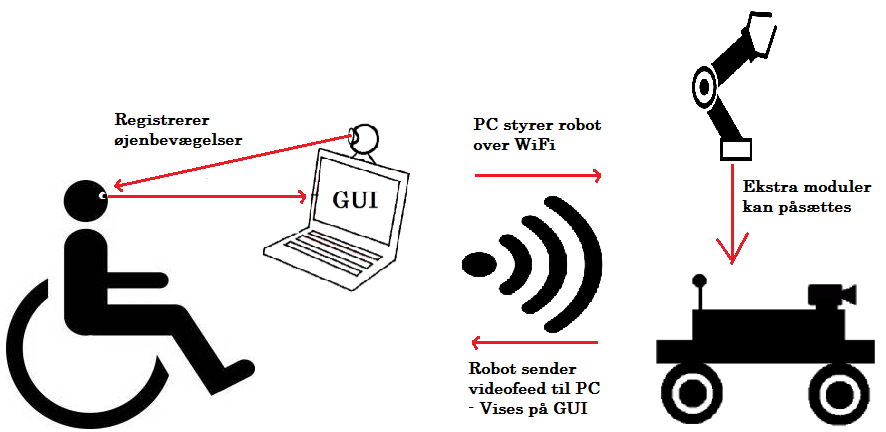
\includegraphics[width = 0.6\textwidth]{Figur/Rigt_billede.png}
	\caption{Sådan virker systemet. Systemet "lytter" og giver en grafisk præsentation af lyden til brugeren, som også kan sætte SD kortet i sin PC og se data der}
	\label{fig:ibd}
\end{figure}


\section{Systemoverblik}
Systemet er bygget op omkring en arduino mega2560. På arduinoen sidder en mikrofon, et ITDB02 Arduino MEGA shield 2.0 med en skærm og en SD kort læser.

På figur \ref{fig:ibd} ses blokdiagrammet for systemet, som viser hvordan mikrofonen, skærmen og SD kort læseren sidder sammen med Arduinoen.

\begin{figure}[H]
	\center
	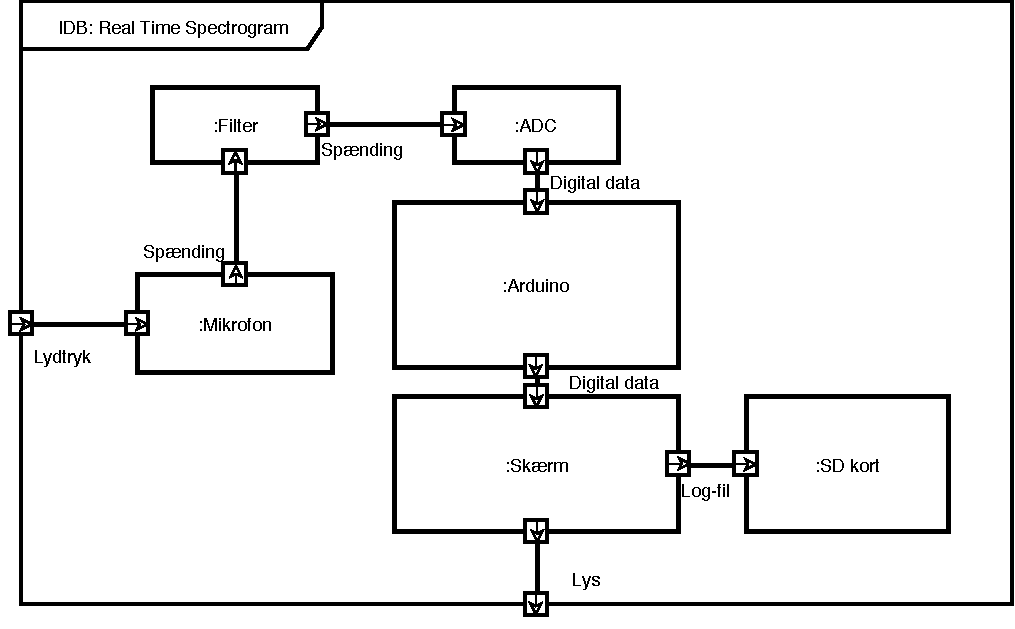
\includegraphics[width = 0.6\textwidth]{Figur/IBD.pdf}
	\caption{Intern blokdiagram for hele systemet}
	\label{fig:ibd}
\end{figure}

Figur \ref{fig:uml} viser klassediagrammet. De forskellige klasser vil blive beskrevet i de afsnit der omhandler delene.

\begin{figure}[H]
	\center
	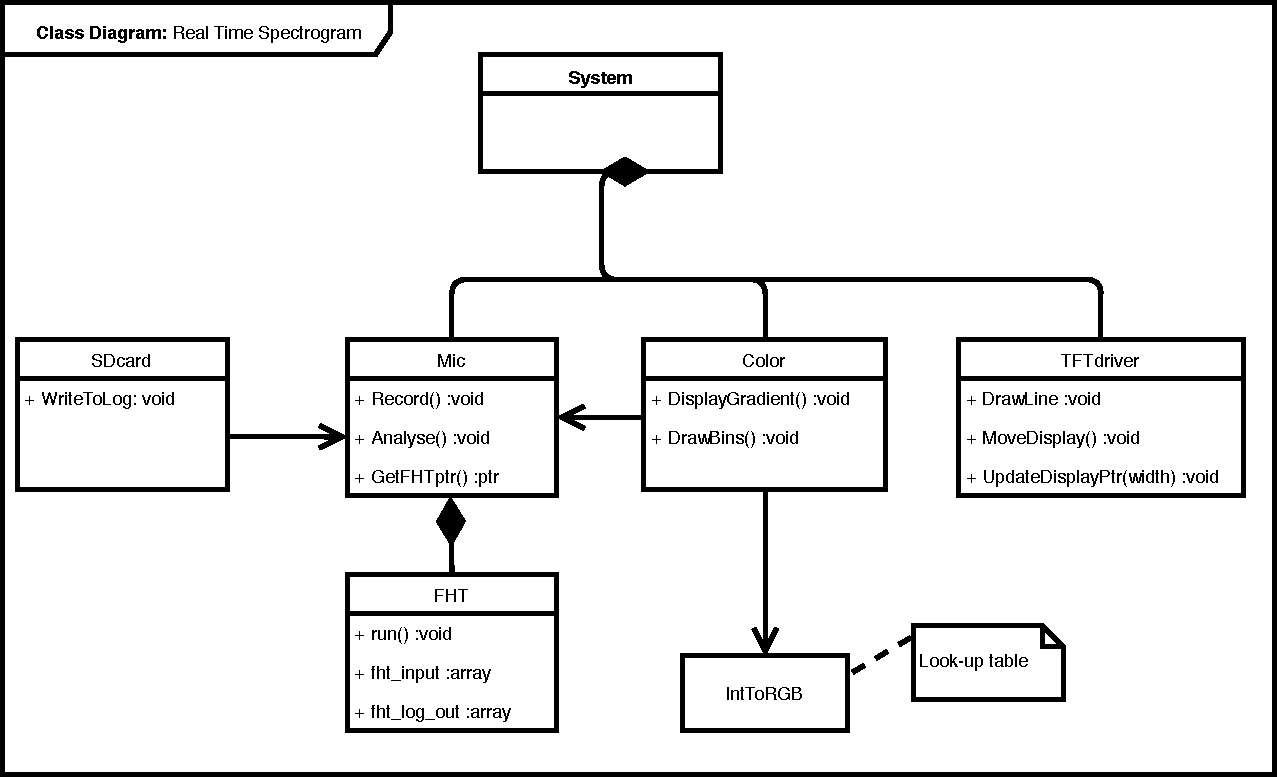
\includegraphics[width = 0.6\textwidth]{Figur/UML.pdf}
	\caption{UML diagram}
	\label{fig:uml}
\end{figure}

%\end{document}